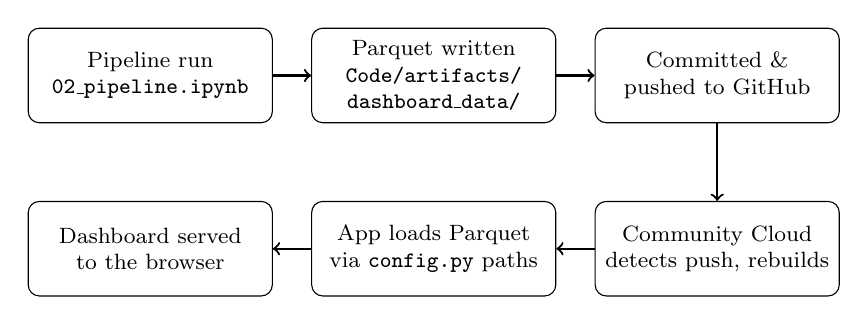
\begin{tikzpicture}[
    box/.style={draw, rounded corners, minimum width=3.1cm, minimum height=1.2cm,
                align=center, font=\footnotesize},
    arr/.style={->, thick}
]
    % top row: local pipeline run through to the GitHub push
    \node[box] (n1) at (0,0)    {Pipeline run\\\texttt{02\_pipeline.ipynb}};
    \node[box] (n2) at (3.6,0) {Parquet written\\\texttt{Code/artifacts/}\\\texttt{dashboard\_data/}};
    \node[box] (n3) at (7.2,0) {Committed \&\\pushed to GitHub};

    % bottom row: Community Cloud picks up the push and serves the app
    \node[box] (n4) at (7.2,-2.2) {Community Cloud\\detects push, rebuilds};
    \node[box] (n5) at (3.6,-2.2) {App loads Parquet\\via \texttt{config.py} paths};
    \node[box] (n6) at (0,-2.2)   {Dashboard served\\to the browser};

    \draw[arr] (n1) -- (n2);
    \draw[arr] (n2) -- (n3);
    \draw[arr] (n3) -- (n4);
    \draw[arr] (n4) -- (n5);
    \draw[arr] (n5) -- (n6);
\end{tikzpicture}
